% =====================================================================
\section{Fundamentos de Li-Fi para a Internet das Coisas}\label{sec:fund-lifi}
% =====================================================================
Esta seção e a próxima foram escritas para leitores que não são especialistas
em comunicações ópticas nem em criptografia. Elas constroem, passo a passo,
todas as ideias necessárias para acompanhar os resultados. Esta trata do lado
da comunicação: o que são os dispositivos de IoT e por que são limitados, como
a luz transporta dados, por que o sinal enfraquece ao longo de uma sala, como
os bits são colocados na luz e o que acontece quando alguns deles chegam
errados. A Tabela~\ref{tab:acronyms} reúne as siglas usadas ao longo do texto.

\begin{table}[!htb]
\caption{Principais siglas e símbolos.}
\label{tab:acronyms}
\centering
\small
\begin{tabular}{ll}
\toprule
termo & significado\\
\midrule
IoT        & Internet das Coisas (pequenos sensores e dispositivos em rede)\\
MCU        & microcontrolador, o pequeno processador de um nó de IoT\\
VLC, Li-Fi & comunicação por luz visível; sua versão em rede\\
LED, PD    & diodo emissor de luz (emissor); fotodiodo (receptor)\\
AP         & ponto de acesso, aqui uma luminária de LED no teto\\
SNR        & relação sinal-ruído, em geral em decibéis (dB)\\
BER        & taxa de erro de bit, fração dos bits recebidos com erro\\
QAM        & modulação de amplitude em quadratura\\
OFDM       & multiplexação por divisão em frequências ortogonais\\
CRC, ARQ   & código de detecção de erros; pedido automático de repetição\\
KEM        & mecanismo de encapsulamento de chaves\\
ML-KEM     & KEM baseado em reticulados, padrão do NIST (FIPS 203)\\
$\ek,\dk,\ct$ & chave de encapsulamento, de desencapsulamento, texto cifrado\\
$R$, $R^{\star}$ & taxa do enlace; taxa de cruzamento (Seção~\ref{sec:cost})\\
\bottomrule
\end{tabular}
\end{table}

\subsection{A Internet das Coisas e suas Limitações}\label{sec:fund-iot}
\emph{Internet das Coisas} (IoT, do inglês \emph{Internet of Things}) é o nome
dado à enorme e crescente população de pequenos dispositivos que medem,
observam ou controlam algo no mundo físico e enviam o resultado por uma rede:
sensores de temperatura e umidade, detectores de presença, medidores
inteligentes, monitores de pacientes, etiquetas de rastreamento em uma fábrica.
Um \emph{nó} típico de IoT tem três partes: um ou mais sensores, um
\emph{microcontrolador} (MCU), que lê os sensores e executa o programa, e um
rádio ou, neste artigo, um transceptor óptico, que o liga a um \emph{ponto de
acesso}. O ponto de acesso encaminha os dados para o restante da rede.

O que distingue um nó de IoT de um celular ou de um notebook é o pouco de que
ele dispõe. A Tabela~\ref{tab:mcus} compara três microcontroladores muito
usados em IoT e em pesquisa com um notebook comum. O processador do nó trabalha
a algumas centenas de megahertz, em vez de vários gigahertz, e tem quilobytes
de memória, em vez de gigabytes. Além disso, costuma ser alimentado por uma
bateria que deve durar meses ou anos; por isso, cada milissegundo que o
processador passa calculando, e cada milissegundo que o transmissor passa
enviando, custa energia.

\begin{table}[!htb]
\caption{Microcontroladores típicos de IoT comparados a um notebook (valores
aproximados).}
\label{tab:mcus}
\centering
\small
\begin{tabular}{lccc}
\toprule
dispositivo & processador & relógio & RAM\\
\midrule
STM32F4 (placa Discovery)  & ARM Cortex-M4 & 168\,MHz & 192\,KB\\
ESP32                      & Xtensa LX6, 2 núcleos & 240\,MHz & 520\,KB\\
Raspberry Pi Pico (RP2040) & ARM Cortex-M0$+$, 2 núcleos & 133\,MHz & 264\,KB\\
\midrule
notebook típico            & x86/ARM, vários núcleos & 3\,GHz & 16\,GB\\
\bottomrule
\end{tabular}
\end{table}

Uma forma útil de pensar no custo de processamento é em \emph{ciclos de
relógio}. Um relógio de $168$\,MHz ``bate'' $168$ milhões de vezes por segundo,
e cada operação simples leva cerca de uma batida. Um algoritmo que precisa de
$C$ ciclos em um processador de frequência $f_{\mathrm{clk}}$ leva, portanto,
\begin{equation}
t = \frac{C}{f_{\mathrm{clk}}}
\label{eq:ciclos}
\end{equation}
segundos. Pela Eq.~\eqref{eq:ciclos}, um algoritmo de $400\,000$ ciclos leva
$400\,000/(168\times10^{6}) \approx 2{,}4$\,ms a $168$\,MHz. A contagem de
ciclos é a forma padrão de comparar programas criptográficos em
microcontroladores porque, ao contrário dos milissegundos, não depende da
frequência configurada. O ARM Cortex-M4, primeiro processador da
Tabela~\ref{tab:mcus}, é a plataforma de referência usual nessas
comparações~\cite{pqm4} e é a que adotamos.

Essas limitações moldam a segurança. Um nó de IoT não consegue executar toda a
pilha de segurança de um navegador, pode permanecer em serviço por uma década e
frequentemente coleta informação sensível: os sinais vitais de um paciente, o
padrão de ocupação de um prédio, o estado de um processo industrial. A
criptografia que ele usa precisa ser barata o bastante para ser executada e
forte o bastante para continuar segura durante toda a vida útil do dispositivo.
É nesse segundo requisito que os computadores quânticos entram na história
(Seção~\ref{sec:fund-quantum}).

\subsection{Comunicação com Luz}\label{sec:fund-light}
A luz visível é radiação eletromagnética, como o rádio, mas de frequência muito
mais alta: cerca de $400$ a $790$\,THz, contra alguns gigahertz do Wi-Fi. A
\emph{comunicação por luz visível} (VLC, \emph{visible light communication})
usa essa luz para transportar dados, e o \emph{Li-Fi} (\emph{light fidelity}) é
a sua versão em rede, na qual cada luminária funciona como um ponto de acesso
sem fio~\cite{haas2016lifi}. O Li-Fi passou recentemente a fazer parte da
família de padrões do Wi-Fi, como IEEE 802.11bb~\cite{ieee80211bb}.

O princípio é simples. Um LED pode ser ligado e desligado, ou ter seu brilho
aumentado e reduzido, milhões de vezes por segundo, muito mais rápido do que o
olho humano percebe; a sala simplesmente parece iluminada de forma constante. O
padrão de variações de brilho codifica os dados, como uma versão muito rápida
de sinalizar com uma lanterna. No receptor, um \emph{fotodiodo}, um pequeno
sensor de luz, produz uma corrente elétrica proporcional à luz que incide sobre
ele, e a eletrônica do receptor converte essa corrente de volta em bits. Esse
esquema chama-se \emph{modulação de intensidade com detecção direta}
(IM/DD)~\cite{kahn1997wireless,ghassemlooy2019owc}. Como o nó não deve iluminar
a sala, o enlace de subida, do nó para o ponto de acesso, normalmente usa luz
infravermelha, que é invisível.

A Tabela~\ref{tab:lifi-wifi} compara Li-Fi e Wi-Fi. Para IoT, três diferenças
importam. O espectro óptico é vasto e não exige licença. A luz não interfere em
equipamentos de rádio, o que é valioso em hospitais, aeronaves e algumas
fábricas. E a luz não atravessa paredes, de modo que uma célula Li-Fi é,
essencialmente, uma sala.

\begin{table}[!htb]
\caption{Li-Fi e Wi-Fi em resumo.}
\label{tab:lifi-wifi}
\centering
\small
\begin{tabular}{lll}
\toprule
 & Wi-Fi & Li-Fi\\
\midrule
portadora            & rádio, 2,4--6\,GHz & luz visível (descida) e infravermelho (subida)\\
espectro             & livre, congestionado & livre, quase sem uso\\
atravessa paredes    & sim & não; uma célula $\approx$ uma sala\\
interferência de rádio & causa e sofre & nenhuma\\
exige visada direta  & não & quase sempre\\
taxas em IoT         & até centenas de Mbit/s & de centenas de kbit/s a Gbit/s\\
\bottomrule
\end{tabular}
\end{table}

É tentador concluir, a partir da última propriedade, que o Li-Fi é seguro por
natureza. Não é. Qualquer pessoa dentro da sala, ou que consiga colocar um
sensor onde a luz chega, recebe exatamente o mesmo sinal que o dispositivo
legítimo~\cite{blinowski2019vlcsec,arfaoui2020plsvlc}. O confinamento reduz
quem pode escutar; não impede a escuta de quem pode. O Li-Fi precisa, portanto,
de criptografia como qualquer outra rede.

\subsection{Como o Sinal Enfraquece ao Longo da Sala}\label{sec:fund-channel}
Um LED não envia sua luz em uma única direção. Ele a espalha em um cone, mais
intenso à frente e mais fraco nas laterais, em um padrão chamado
\emph{lambertiano}. Um receptor diretamente sob a luminária recebe, por isso,
muito mais luz do que um receptor próximo à parede, por dois motivos: está mais
perto e está na parte mais intensa do cone. O modelo padrão desse efeito
fornece a fração da luz emitida que chega ao receptor, chamada \emph{ganho do
canal}~\cite{kahn1997wireless,komine2004vlc}:
\begin{equation}
h = \frac{(m+1)A_{\mathrm{pd}}}{2\pi d^{2}}\cos^{m}(\phi)\cos(\psi),
\qquad 0\le\psi\le\Psi_{\mathrm{fov}}.
\label{eq:gain}
\end{equation}
Cada fator da Eq.~\eqref{eq:gain} tem um significado simples. O termo
$1/d^{2}$ diz que a luz se espalha: dobrar a distância $d$ divide por quatro a
potência recebida, a mesma regra que faz uma lâmpada parecer mais fraca quanto
mais longe se está. O termo $\cos^{m}(\phi)$ descreve o cone: $\phi$ é o ângulo
entre o eixo do LED e a direção do receptor, e o expoente $m$, chamado
\emph{ordem lambertiana}, é maior para um feixe estreito e menor para um feixe
largo. Ele é calculado a partir do ângulo $\Phi_{1/2}$ em que o brilho do LED
cai à metade~\cite{kahn1997wireless}:
\begin{equation}
m = -\frac{\ln 2}{\ln\cos\Phi_{1/2}}.
\label{eq:lambert}
\end{equation}
Para o LED deste trabalho, modelado de acordo com ~\cite{almoliki2022lci}, com $\Phi_{1/2}=70^{\circ}$, a
Eq.~\eqref{eq:lambert} fornece $m\approx0{,}65$. O termo $\cos(\psi)$ leva em
conta a luz que chega inclinada ao detector, e $A_{\mathrm{pd}}$ é a área do
detector: um detector maior coleta mais luz. Por fim, o receptor só enxerga a
luz que chega dentro do seu campo de visão $\Psi_{\mathrm{fov}}$; fora dele, o
ganho é zero.

A luz recebida nunca é perfeitamente limpa. A luz do sol e de outras lâmpadas
acrescenta uma flutuação aleatória à corrente do fotodiodo (\emph{ruído
shot}), e a própria eletrônica do receptor acrescenta mais (\emph{ruído
térmico}). A qualidade com que o receptor recupera os dados depende de quão
forte é o sinal em comparação com esse ruído, grandeza chamada \emph{relação
sinal-ruído} (SNR). A SNR é quase sempre expressa em decibéis (dB), uma escala
logarítmica em que cada $10$\,dB correspondem a um fator de dez: uma SNR de
$20$\,dB significa que a potência do sinal é $100$ vezes a do ruído, e
$30$\,dB, $1000$ vezes. Para o cenário modelado neste trabalho, o ruído é aproximadamente o mesmo em toda a sala ~\cite{almoliki2022lci}, 
enquanto o sinal segue a Eq.~\eqref{eq:gain}, de modo que a SNR em uma posição $(x,y)$
pode ser escrita em relação à SNR no centro, $\mathrm{SNR}_{c}$:
\begin{equation}
\mathrm{SNR}(x,y) = \mathrm{SNR}_{c} + 20\log_{10}\frac{h(x,y)}{h(0,0)} \ \text{dB},
\label{eq:snr}
\end{equation}
em que o fator $20$ (e não $10$) aparece porque a potência elétrica do sinal é
proporcional ao quadrado da potência óptica
recebida~\cite{kahn1997wireless}. Na sala modelada aqui, a
Eq.~\eqref{eq:snr} indica que a SNR cai $\val{PosSnrDrop}$\,dB, de
$\val{PosCentreSnr}$\,dB sob a luminária para $\val{PosEdgeSnr}$\,dB junto à
parede (Figura~\ref{fig:snr}). Como mostram as próximas subseções, essa queda
aparentemente modesta tem grandes consequências.

\subsection{Dos Bits à Luz: Modulação}\label{sec:fund-mod}
\emph{Modulação} é a regra que transforma bits em um sinal físico. A regra
óptica mais simples, o chaveamento liga-desliga (\emph{on--off keying}), envia
um $1$ como luz e um $0$ como escuro, um bit por intervalo de tempo. Enlaces
mais rápidos enviam vários bits por intervalo usando vários níveis.

A \emph{modulação de amplitude em quadratura} (QAM) leva essa ideia a duas
dimensões. Cada grupo de $b$ bits é mapeado em um de $M=2^{b}$ pontos de uma
grade chamada \emph{constelação}; a Figura~\ref{fig:qam} mostra a 16-QAM, em que
cada ponto representa $4$ bits. O receptor mede um ponto, mas o ruído o desloca
um pouco de onde foi enviado, e o receptor então escolhe o ponto da grade mais
próximo. Se o ruído for grande o bastante para empurrar a medida além da linha
do meio do caminho até um ponto vizinho, ocorre um \emph{erro de símbolo}. Os
rótulos são dispostos em \emph{código de Gray}, de modo que pontos vizinhos
diferem em apenas um bit; assim, o erro de símbolo mais provável corrompe só um
dos $b$ bits. Mais pontos por constelação significam mais bits por símbolo, mas
também pontos mais próximos entre si e, portanto, mais erros para a mesma SNR.
Este artigo usa 32-QAM, que transporta $5$ bits por símbolo.

% Constelação 16-QAM com rótulos de Gray e um ponto recebido com ruído.
\begin{figure}[!htb]
\centering
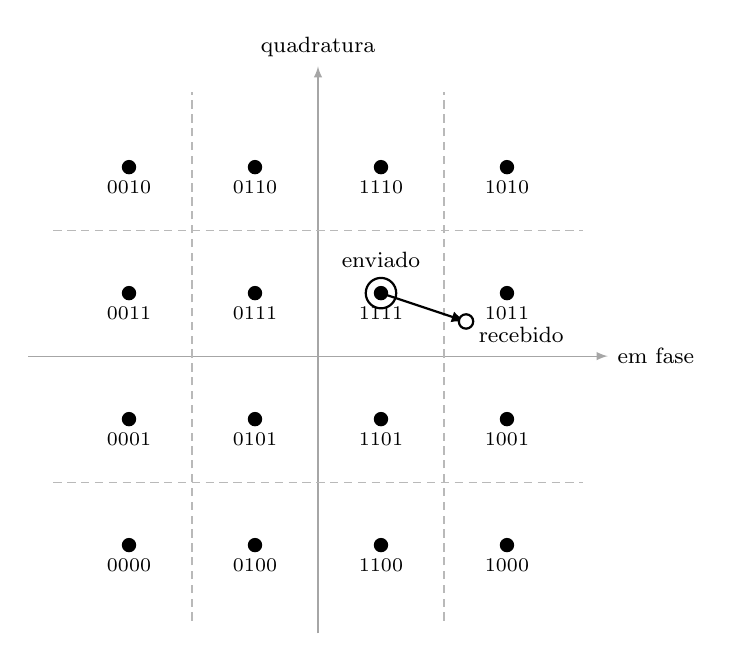
\begin{tikzpicture}[x=0.8cm,y=0.8cm,font=\footnotesize,>=latex]
  % eixos
  \draw[->,gray!70] (-4.6,0) -- (4.6,0) node[right,black] {em fase};
  \draw[->,gray!70] (0,-4.4) -- (0,4.6) node[above,black] {quadratura};
  % fronteiras de decisão
  \foreach \v in {-2,2}{
    \draw[densely dashed,gray!55] (\v,-4.2) -- (\v,4.2);
    \draw[densely dashed,gray!55] (-4.2,\v) -- (4.2,\v);}
  % pontos em código de Gray: amplitude -> rótulo de 2 bits
  \def\lab#1{\ifcase#1 00\or 01\or 11\or 10\fi}
  \foreach \i/\x in {0/-3,1/-1,2/1,3/3}{
    \foreach \j/\y in {0/-3,1/-1,2/1,3/3}{
      \fill (\x,\y) circle (2.6pt);
      \node[below=1.5pt,font=\scriptsize] at (\x,\y) {\lab{\i}\lab{\j}};
    }}
  % ponto enviado, ponto recebido com ruído e o erro
  \draw[black,thick] (1,1) circle (5.5pt);
  \node[anchor=south,fill=white,inner sep=1pt] at (1,1.36) {enviado};
  \draw[->,thick] (1,1) -- (2.35,0.55);
  \fill[white,draw=black,thick] (2.35,0.55) circle (2.6pt);
  \node[anchor=north west,inner sep=1pt] at (2.5,0.52) {recebido};
\end{tikzpicture}
\caption{16-QAM: cada ponto representa 4 bits. As linhas tracejadas são as
fronteiras de decisão. Aqui \texttt{1111} é enviado, o ruído empurra a medida
para além de uma fronteira, e o receptor decide \texttt{1011}. Como os rótulos
seguem um código de Gray, pontos vizinhos diferem em um único bit.}
\label{fig:qam}
\end{figure}


Enviar símbolos QAM um após o outro em alta taxa traz um problema em ambientes
fechados: a luz chega ao receptor por vários caminhos, diretamente e após
refletir nas paredes, e, em altas taxas, essas cópias atrasadas ``borram'' cada
símbolo sobre o seguinte. A \emph{multiplexação por divisão em frequências
ortogonais} (OFDM) evita isso dividindo um fluxo rápido em muitos fluxos lentos,
cada um transportado em sua própria frequência, a \emph{subportadora}, e todos
enviados em paralelo~\cite{armstrong2013ofdm}. Cada fluxo lento quase não é
afetado pelo borrão. A divisão e a recombinação são feitas com a transformada
rápida de Fourier (FFT) e a sua inversa (IFFT), e um curto \emph{prefixo
cíclico}, uma cópia do final de cada símbolo OFDM colocada no seu início,
absorve o borrão que restar.

A luz impõe duas restrições que o rádio não tem. O brilho de um LED é um único
número real e não pode ser negativo. A IFFT normalmente produz um sinal
complexo e bipolar; por isso, são feitos dois ajustes. Primeiro, as $N$
subportadoras, de símbolos $X_0,\dots,X_{N-1}$, são preenchidas em pares
espelhados~\cite{armstrong2013ofdm}:
\begin{equation}
X_{N-k} = X_k^{*}, \qquad X_0 = X_{N/2} = 0,
\label{eq:hermitian}
\end{equation}
em que $X_k^{*}$ é o complexo conjugado de $X_k$. A propriedade da
Eq.~\eqref{eq:hermitian}, chamada \emph{simetria hermitiana}, torna a saída
real. O preço é que apenas metade das $N$ subportadoras transporta dados
independentes, menos as duas que precisam ficar vazias. Segundo, soma-se um
\emph{nível DC} constante para que o sinal fique quase todo positivo, e os
poucos picos que ainda ficarem negativos ou excessivamente altos são
\emph{ceifados} (\emph{clipping}). Esse esquema chama-se \emph{OFDM óptico com
polarização DC} (DCO-OFDM)~\cite{armstrong2013ofdm}, e a Figura~\ref{fig:ofdm}
mostra a cadeia completa.

% Cadeia de transmissão e recepção DCO-OFDM.  TikZ puro.
\begin{figure}[!htb]
\centering
\begin{tikzpicture}[
  font=\footnotesize,
  blk/.style={draw,rounded corners=1.5pt,align=center,inner sep=3pt,
              minimum height=10mm,minimum width=15mm,fill=black!4},
  opt/.style={blk,fill=black!14},
  every path/.style={>=latex,->},
  node distance=3.6mm
]
% ------------------------------ transmissor ------------------------------
\node (bits) {bits};
\node[blk,right=of bits]   (qam)  {mapa\\QAM};
\node[blk,right=of qam]    (herm) {simetria\\hermit.};
\node[blk,right=of herm]   (ifft) {IFFT};
\node[blk,right=of ifft]   (cp)   {insere\\prefixo};
\node[blk,right=of cp]     (dc)   {nível DC\\+ ceifam.};
\node[opt,right=of dc]     (led)  {LED};
\draw (bits) -- (qam);
\draw (qam) -- (herm);
\draw (herm) -- (ifft);
\draw (ifft) -- (cp);
\draw (cp) -- (dc);
\draw (dc) -- (led);
\node[anchor=south west,font=\footnotesize\itshape,inner sep=1pt]
     at ([yshift=2.5mm]qam.north west) {transmissor};

% --------------------------------- canal ---------------------------------
\node[draw,dashed,rounded corners=1.5pt,align=center,inner sep=3pt,
      below=6mm of led] (ch)
     {$h(x,y)$\\$+$ ruído};
\draw (led) -- (ch);

% -------------------------------- receptor --------------------------------
\node[opt,below=6mm of ch]  (pd)   {PD};
\node[blk,left=of pd]       (rcp)  {remove\\prefixo};
\node[blk,left=of rcp]      (fft)  {FFT};
\node[blk,left=of fft]      (eq)   {equali-\\zação};
\node[blk,left=of eq]       (sel)  {mantém\\$k<\!N/2$};
\node[blk,left=of sel]      (dem)  {demapa\\QAM};
\node[left=of dem]          (obits){bits};
\draw (ch) -- (pd);
\draw (pd) -- (rcp);
\draw (rcp) -- (fft);
\draw (fft) -- (eq);
\draw (eq) -- (sel);
\draw (sel) -- (dem);
\draw (dem) -- (obits);
\node[anchor=north west,font=\footnotesize\itshape,inner sep=1pt]
     at ([yshift=-2.5mm]dem.south west) {receptor};
\end{tikzpicture}
\caption{Cadeia DCO-OFDM. A simetria hermitiana da Eq.~\eqref{eq:hermitian}
torna real a saída da IFFT, para que ela possa acionar um LED; o nível DC e o
ceifamento a tornam não negativa. Só $N/2-1$ subportadoras transportam dados, o
que fixa a carga de um símbolo na Eq.~\eqref{eq:bsym}. Os blocos sombreados são
ópticos.}
\label{fig:ofdm}
\end{figure}


Juntando as peças~\cite{armstrong2013ofdm}, conclui-se que cada símbolo
DCO-OFDM transporta
\begin{equation}
B_{\mathrm{sym}} = \left(\tfrac{N}{2}-1\right)\log_2 M \ \text{bits}.
\label{eq:bsym}
\end{equation}
Com $N=512$ subportadoras e 32-QAM, a Eq.~\eqref{eq:bsym} resulta em
$(256-1)\times5 = \val{BitsPerSymbol}$ bits, cerca de $159$ bytes por símbolo
OFDM.

O ceifamento distorce ligeiramente o sinal. Um resultado conhecido como
teorema de Bussgang permite tratar essa distorção como uma pequena e previsível
perda de sinal, de fator $\alpha$, somada a um ruído adicional de potência
$\sigma_c^{2}$~\cite{dimitrov2013information}. Se $\gamma$ é a SNR sem
ceifamento, em escala linear, a SNR efetiva passa a ser
\begin{equation}
\gamma_{\mathrm{ef}} = \frac{\alpha^{2}}{\gamma^{-1} + \sigma_c^{2}}.
\label{eq:gammaeff}
\end{equation}
Para o ceifamento usado aqui, em $\pm3{,}2$ desvios-padrão, $\alpha\approx0{,}999$
e $\sigma_c^{2}\approx1{,}9\times10^{-4}$, de modo que a
Eq.~\eqref{eq:gammaeff} quase não altera a SNR nas condições estudadas.

\subsection{Quando os Bits Chegam Errados: a Taxa de Erro de Bit}\label{sec:fund-ber}
A \emph{taxa de erro de bit} (BER) é a fração dos bits recebidos que estão
errados. Uma BER de $10^{-5}$ significa um bit errado a cada $100\,000$. Ela
depende da SNR e da constelação e, para QAM com código de Gray, é bem
aproximada por~\cite{proakis2008digital}
\begin{equation}
P_b \simeq \frac{\bar{n}\,h_{\mathrm{nn}}}{\log_2 M}\,
           Q\!\left(d_{\min}\sqrt{\gamma_{\mathrm{ef}}/2}\right),
\label{eq:ber}
\end{equation}
em que $\gamma_{\mathrm{ef}}$ é a SNR efetiva da Eq.~\eqref{eq:gammaeff},
$d_{\min}$ é a distância entre pontos vizinhos da constelação, $\bar{n}$ é o
número médio de vizinhos de um ponto e $h_{\mathrm{nn}}$ é o número de bits que
diferem entre vizinhos (cerca de um, graças ao código de Gray). A função
$Q(\cdot)$ é a probabilidade de um ruído gaussiano exceder certo número de
desvios-padrão; o que importa aqui é que ela cai muito depressa à medida que
seu argumento cresce.

Essa queda abrupta é a razão de alguns decibéis fazerem tanta diferença. A
Figura~\ref{fig:snr} aplica as Eqs.~\eqref{eq:snr} e~\eqref{eq:ber} ao longo da
sala. Sob a luminária, a $\val{PosCentreSnr}$\,dB, a BER é de cerca de
$10^{-8}$: um bit errado a cada cem milhões. Junto à parede, apenas
$\val{PosSnrDrop}$\,dB abaixo, ela é de $\val{PosEdgeBer}$, cerca de três bits
errados a cada mil, mais de cem mil vezes maior. Como mostra a
Seção~\ref{sec:results}, essa diferença domina o custo da troca de chaves na
borda da sala.

% SNR e BER ao longo da sala (y = 0), a partir do modelo do enlace.
\begin{figure}[!htb]
\centering
\begin{tikzpicture}
\begin{groupplot}[
  group style={group size=1 by 2, vertical sep=0.6cm, x descriptions at=edge bottom},
  width=0.8\textwidth, height=4.6cm,
  xmin=-2.5, xmax=2.5, grid=both, grid style={gray!18},
  label style={font=\small}, tick label style={font=\footnotesize},
  xlabel={posição do receptor $x$ (m), com $y=0$},
]
\nextgroupplot[ylabel={SNR (dB)}, ymin=17, ymax=26]
  \addplot[black,line width=0.9pt] table[x=x,y=snr_db] {data/handshake_position.dat};
  \node[font=\footnotesize,anchor=north] at (axis cs:0,22.6) {sob a luminária};
  \draw[gray!60,->] (axis cs:0,22.7) -- (axis cs:0,24.7);
  \node[font=\footnotesize,anchor=south west] at (axis cs:-2.45,17.3) {parede};
\nextgroupplot[ymode=log, ylabel={BER}, ymin=1e-9, ymax=1e-2,
  ytick={1e-8,1e-6,1e-4,1e-2}]
  \addplot[black,line width=0.9pt] table[x=x,y=ber] {data/handshake_position.dat};
  \addplot[gray!70,densely dashed,domain=-2.5:2.5] {1e-5};
  \node[font=\footnotesize,anchor=south,gray!40!black] at (axis cs:0,1.2e-5)
    {$10^{-5}$: um bit errado em $100\,000$};
\end{groupplot}
\end{tikzpicture}
\caption{Qualidade do sinal ao longo da sala, pelas Eqs.~\eqref{eq:snr}
e~\eqref{eq:ber}. A SNR cai apenas $\val{PosSnrDrop}$\,dB do centro até a
parede, mas a BER sobe cinco ordens de grandeza, de cerca de
$10^{\val{PosCentreBerExp}}$ para $\val{PosEdgeBer}$.}
\label{fig:snr}
\end{figure}


\subsection{Pacotes, Verificação de Erros e Retransmissão}\label{sec:fund-arq}
Enlaces reais não enviam um único fluxo longo de bits; enviam \emph{pacotes}.
Uma mensagem longa demais para um pacote é cortada em \emph{fragmentos}, cada
um enviado com um pequeno \emph{cabeçalho} que indica qual fragmento é e
carrega um código de verificação. O código usado quase universalmente, a
verificação de redundância cíclica (CRC), é um código curto calculado a partir
do conteúdo do fragmento. O receptor o recalcula; se os dois valores diferem,
ao menos um bit foi corrompido, e o fragmento é descartado.

Um fragmento descartado precisa ser enviado de novo. A forma mais simples de
organizar isso é o \emph{pedido automático de repetição do tipo
pare-e-espere} (ARQ \emph{stop-and-wait}): o emissor transmite um fragmento e
aguarda uma curta confirmação; se ela não chega, envia o mesmo fragmento outra
vez. Cada retransmissão custa tempo de transmissão.

A probabilidade de um fragmento chegar intacto decorre diretamente da BER. Se
cada um dos seus $n$ bits está errado, de forma independente, com probabilidade
$P_b$, todos os $n$ bits estão certos com
probabilidade~\cite{bertsekas1992data}
\begin{equation}
P_{\mathrm{ok}} = (1-P_b)^{n}.
\label{eq:psurv}
\end{equation}
Um fragmento com $128$ bytes de dados e $8$ bytes de cabeçalho tem
$n = 8\times136 = 1088$ bits. Pela Eq.~\eqref{eq:psurv}, com $P_b=10^{-5}$ ele
sobrevive com probabilidade $0{,}989$, e retransmissões são raras. Com
$P_b=10^{-3}$, sobrevive com probabilidade $(0{,}999)^{1088}\approx0{,}34$:
dois em cada três fragmentos se perdem e precisam ser reenviados. Esse é o
mecanismo por trás do efeito da posição mostrado na Seção~\ref{sec:results}, e
ele também explica por que fragmentos menores ajudam em um enlace ruim: menos
bits por fragmento significam mais chance de cada um chegar inteiro.
